\documentclass[a4paper,14pt]{extarticle}

%%% Решение проблемы копирования текста в буфер кракозябрами
\usepackage{cmap}   % Улучшенный поиск русских слов в полученном pdf-файле
\usepackage{textcomp}
\usepackage[T1,T2A]{fontenc}                    % Поддержка русских букв
% \usepackage{pscyr}  % Подключение pscyr
\usepackage[utf8]{inputenc}         % Кодировка utf8
\usepackage[english, russian]{babel} % Языки: русский, английский

\usepackage[left=3cm, right=1.5cm, top=2cm, bottom=2cm]{geometry}

\usepackage{setspace}
\onehalfspacing{}

\usepackage[center]{titlesec}
\usepackage[justification=centering,font=small]{caption}

\usepackage{indentfirst}
\setlength{\parindent}{20pt}

\usepackage{fancyhdr}
\setlength{\headheight}{17.0pt}
\pagestyle{fancy}
\fancyhf{}
\fancyhead[C]{\thepage}
\renewcommand{\headrulewidth}{0pt}

\usepackage[normalem]{ulem}

\hyphenpenalty=0

\usepackage[hidelinks]{hyperref}

\usepackage{graphicx}
\graphicspath{{images/}}
\usepackage{pdfpages}
\usepackage{subcaption}

\usepackage{miller}
\newcommand{\unit}[1]{ \ \text{#1}}
\newcommand{\degree}{^\circ}
\newcommand{\celcius}{^\circ \text{C}}
\newcommand{\YEu}{${(\text{Y}_{1-x}\text{Eu}_x)}_2\text{O}_3$}
\newcommand{\range}[2]{[#1\div#2]}

\usepackage{forloop}
\newcounter{x}
\newcommand{\Repeat}[2]{\forloop{x}{0}{\value{x} < #1}{#2}}
\newcommand{\writedate}{<<\Repeat{2}{\ldots}>>\Repeat{5}{\ldots}2025г.}

\usepackage{csquotes}
\bibliographystyle{gost-numeric.bbx}
\usepackage[backend=biber,
citestyle=gost-numeric,
bibstyle=gost-numeric,
sorting=none,
]{biblatex}
\addbibresource{bibliography.bib}

\usepackage{multirow}

\usepackage{amsmath}
\usepackage{tensor}

\begin{document}
\begin{titlepage}
\thispagestyle{empty}
\begin{spacing}{1.15}
\footnotesize
\begin{center}
    МИНИСТЕРСТВО НАУКИ И ВЫСШЕГО ОБРАЗОВАНИЯ РОССИЙСКОЙ ФЕДЕРАЦИИ
    \vspace{20pt}

    ФЕДЕРАЛЬНОЕ ГОСУДАРСТВЕННОЕ АВТОНОМНОЕ ОБРАЗОВАТЕЛЬНОЕ\\
    УЧРЕЖДЕНИЕ ВЫСШЕГО ОБРАЗОВАНИЯ
    \vspace{6pt}

    «НОВОСИБИРСКИЙ НАЦИОНАЛЬНЫЙ ИССЛЕДОВАТЕЛЬСКИЙ ГОСУДАРСТВЕННЫЙ УНИВЕРСИТЕТ» (НОВОСИБИРСКИЙ ГОСУДАРСТВЕННЫЙ УНИВЕРСИТЕТ, НГУ)
    \vspace{10pt}
\end{center}
Факультет \uline{\textbf{ФИЗИЧЕСКИЙ}}
\vspace{10pt}

\noindent
Кафедра \uline{\textbf{ФИЗИЧЕСКИХ МЕТОДОВ ИССЛЕДОВАНИЯ ТВЕРДОГО ТЕЛА}}
\vspace{8mm}

\noindent
Направление подготовки \uline{\textbf{03.03.02 ФИЗИКА}}
\vspace{10pt}

\noindent
Образовательная программа: \uline{\textbf{БАКАЛАВРИАТ}}
\vspace{8mm}
\begin{center}
    \textbf{ВЫПУСКНАЯ КВАЛИФИКАЦИОННАЯ РАБОТА}

    \textbf{(научно-исследовательский формат)}
    \vspace{8mm}

    \uline{\hfill Кудрявцева Артема Леонидовича \hfill}

    $_\text{(Фамилия, Имя, Отчество автора)}$
    \vspace{8mm}
\end{center}
Тема работы \uline{Разработка методики определения параметров элементарной ячейки монокристаллов на дифрактометре, оснащенном двумерным детектором\hfill}
\vfill

\noindent
\textbf{«К защите допущена»}

\noindent
Заведующий кафедрой \hfill \textbf{Научные руководители}
\vspace{10pt}

\noindent
д.~ф.-м.~н., профессор \hfill д.~ф.-м.~н., профессор
\vspace{10pt}

\noindent
г.~н.~с. ИК СО РАН \hfill г.~н.~с. ИНХ СО РАН
\vspace{10pt}

\noindent
Цыбуля~С.В./\writesign{}\hfill{}Громилов~С.А./\writesign{}

\noindent
$_\text{(фамилия И., О.) / (подпись, МП)}$ \hfill $_\text{(фамилия И., О.) / (подпись, МП)}$
\vspace{10pt}

\noindent
\writedate\hfill м.~н.~с. ИНХ СО РАН
\vspace{10pt}

\noindent
\hfill Серебренникова~П.С./\writesign{}

\noindent
\hfill $_\text{(фамилия И., О.) / (подпись, МП)}$
\vspace{10pt}

\noindent
\hfill\writedate{}
\vspace{8mm}

\hfill Дата защиты:\writedate{}
\vspace{8mm}

\begin{center}
    Новосибирск, 2025
\end{center}

\end{spacing}
\end{titlepage}
\setcounter{page}{2}
\tableofcontents
\section{Введение}

Точность измерения параметров элементарной ячейки (ПЭЯ) монокристаллов на дифрактометрах, оборудованных 2D-детекторами, обсуждается достаточно активно~\cite{Herbstein:2000,Waterman:2010,Dudka:2010,Henn:2019,Taylor:1986,Serebrennikova:2021}.
В работе~\cite{Dudka:2017} проблема сформулирована следующим образом: <<\ldotsпопытки получить воспроизводимые значения параметров элементарных ячеек монокристаллов при повторных исследованиях или исследовать зависимости этих параметров от температуры или давления могут привести к разочарованию>>.
К этому можно добавить, что это утверждение справедливо и при сопоставлении данных рентгеноструктурного анализа (РСтА) монокристаллов и дифрактометрии поликристаллов.
Трудно перечислить все подходы, предложенные для минимизации ошибок измерения ПЭЯ монокристаллов.
Среди последних обзоров на эту тему можно указать~\cite{Galdecka:2006,Lider:2020}.
Возможности методик с использованием внешнего или внутреннего эталонов на ряде примеров продемонстрированы в работах~\cite{Gromilov:2022,Panchenko:2022,Panchenko:2023,Serebrennikova:2023,Serebrennikova:2022}.
Особо следует отметить, что эти методики ориентированы на исследование малых монокристаллов (т.е. имеющих размер меньше первичного пучка), пригодных для проведения РСтА.
Пробоотбор подходящих для исследования образцов такой же, как и для РСтА --- требуется совершенный кристаллик с линейными размерами <0.1~мм.
Дополнительное требование --- наличие рефлексов с разрешенным дублетом, если оно выполняется, то при использовании рефлексов с $2\theta \approx 120\degree$ и гониометров с точностью $0.005\degree$ можно рассчитывать на измерение межплоскостных расстояний с относительной ошибкой не хуже $\Delta d / d = 5 \cdot 10^{-5}$.
Не во всех случаях использование внутреннего эталона удобно, т.к. требует дополнительных усилий при подготовке и определении ориентации одновременно обоих кристаллов, а также приводит к уменьшению интенсивности и взаимному экранированию~\cite{Serebrennikova:2022}.
Использование внешнего эталона обычно вызывает вопросы об эквивалентности установки образцов.
В этом плане развитие безэталонных методик имеет свои перспективы.

Классической безэталонной методикой измерения ПЭЯ является схема Бонда~\cite{Bond:1960}, в основе которой лежат два основных фактора – наличие точного гониометра (достаточно одноосного) и сориентированной определенным образом монокристаллической пластинки (см. рис.~\ref{fig:bond}а).
Методика хорошо себя проявила на малых кристаллах~\cite{Lisoivan:1988}, хотя при использовании одноосных гониометров в случае кристаллов средних и низших сингоний требуется переклейка кристалла.
Современные монокристальные дифрактометры оснащаются моторизированными гониометрами позволяющими поворачивать образец вокруг двух- или трех осей, что делает их подходящими для реализации схемы Бонда.
Причем эту схему можно реализовать как на больших ориентированных монокристаллических пластинах, так и на малых кристаллах.
Если при измерениях на больших кристаллах (см. рис.~\ref{fig:bond}а) угол $2\theta = \omega_+ - \omega_-$ свободен от ошибок, связанных со смещением образца с оси гониометра, то во втором необходимо учитывать возможное смещение, т.е. эксцентриситет.
Эксцентриситет зависит как от размера сферы сведения осей (\textit{sphere of confusion}), так и точности центрирования образца.
Подходы к экспериментальному учету эксцентриситета малых монокристаллов достаточно хорошо проработаны в литературе см., например,~\cite{Ponomarev:1969,King:1979}.

\begin{figure}[ht!]
    \centering
    \begin{subfigure}{0.5\textwidth}
    \centering
    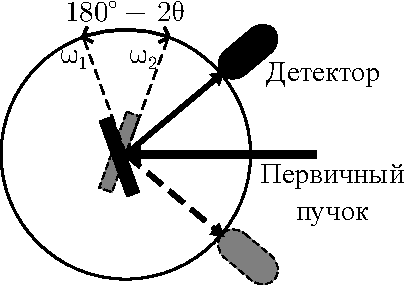
\includegraphics[]{bond.pdf}
    \caption{}%
    \label{fig:bond}
    \end{subfigure}%
    \begin{subfigure}{0.5\textwidth}
    \centering
    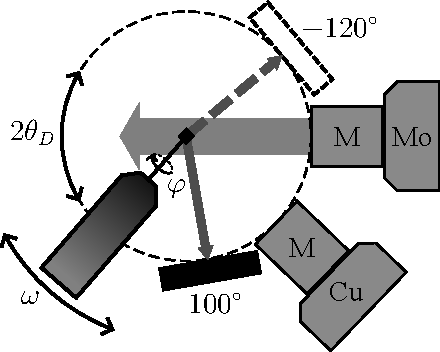
\includegraphics[]{our_bond.pdf}
    \caption{}%
    \label{fig:our_bond}
    \end{subfigure}
    \caption{Схемы эксперимента для учета эксцентриситета образца.}%
\end{figure}

Кроме этого, точность измерения ПЭЯ зависит от точности гониометра.
В паспорте сейчас обычно указывают лишь воспроизводимость установки углов, и не указывают значение самой погрешности.
Другие ошибки, возникающие при использовании серийных приборов, ориентированных на проведение РСтА, обусловлены значительной расходимостью первичного пучка (на уровне нескольких десятых градуса).
На точность измерений влияет и общая компоновка гониометра: при горизонтальном расположении рентгеновской трубки доступные для съемки углы $2\theta$ значительно ограничены.
Использование 2D-детектора также ограничивает углы $2\theta$, а также предполагает обработку двумерных профилей, что вносит свои нюансы в определение положения максимума, особенно при неполном разрешении дублета.
В основе точности измерений ПЭЯ в схеме Бонда лежит значение использованной длины волны, далее будут использованы рекомендованные значения $\lambda \text{Mo} K \alpha_1 = 0.70931715 (41)\unit{\AA}$ и $\lambda \text{Mo} K \alpha_2 = 0.713607 (12)\unit{\AA}$~\cite{Deslattes:1985}.

Проведение измерений ПЭЯ с максимально достижимой точностью всегда было особым разделом рентгенографии.
Уже для первых дифрактометров был предложен ряд подходов к учету основных приборных ошибок~\cite{Ponomarev:1969}. В~\cite{King:1979} предложен метод учета основных ошибок по результатам съемки 8 рефлексов на приборе, оснащенном четырехкружным гониометром и точечным детектором.
Цель настоящей работы --- оценка и учет ошибок измерений ПЭЯ, связанных с эксцентриситетом образца, в схеме Бонда на современных дифрактометрах.
Для этого логично привлечь эталонные образцы, для которых ПЭЯ известны с хорошей точностью.

% chktex-file 44
\section{Экспериментальная часть}
\subsection{Описание установки}
Рентгенографические эксперименты проводились на монокристальном дифрактометре Bruker D8 Venture (см. рисунок~\ref{fig:D8_photo}).
Его оборудование и характеристики:
\begin{itemize}
    \item Микрофокусная трубка Incoatec $I \mu S \ 3.0$
    \begin{itemize}
        \item $\text{Cu} K\alpha$ и $\text{Mo} K\alpha$ излучение
        \item Монохроматизация и коллимация с помощью многослойных зеркал Монтеля
        \item Диаметр пучка $110\unit{мкм}$
        \item Расходимость $0.3\degree$
    \end{itemize}
    \item Двумерный детектором PHOTON III
    \begin{itemize}
        \item CMOS-технология матрицы
        \item Разрешение $768 \times 1024$ пикселей
        \item Размер пикселя $135 \times 135\unit{мкм}^2$
        \item Ручная установка расстояния до образца
    \end{itemize}
    \item Трехкружный гониометр FIXED-CHI
    \begin{itemize}
        \item Гониометр использует эйлерову геометрию
        \item Автоматическая регулировка углов $\varphi$ и $\omega$ для образца и $2\theta_D$ для детектора
        \item Угол $\chi$ фиксирован и равен $54.7112\degree$
        \item Воспроизводимость установки углов $0.0001\degree$
        \item Точность установки углов $0.004\degree$\footnote{Паспортная точность установки углов не указана, но согласно результатам измерения эталонного образца на порошковом дифрактометре Bruker D8 Advance, оснащенном аналогичным гониометром, она не хуже $0.005\degree$.}
    \end{itemize}
    \item Температурная приставка Oxford Cryostream 800Plus
    \begin{itemize}
            \item Стабильность поддержания температуры $0.2\unit{К}$
    \end{itemize}
    \item Управление прибором средствами программного пакета APEX3~\cite{Bruker:2019}
\end{itemize}

\begin{figure}[ht!]
    \centering
    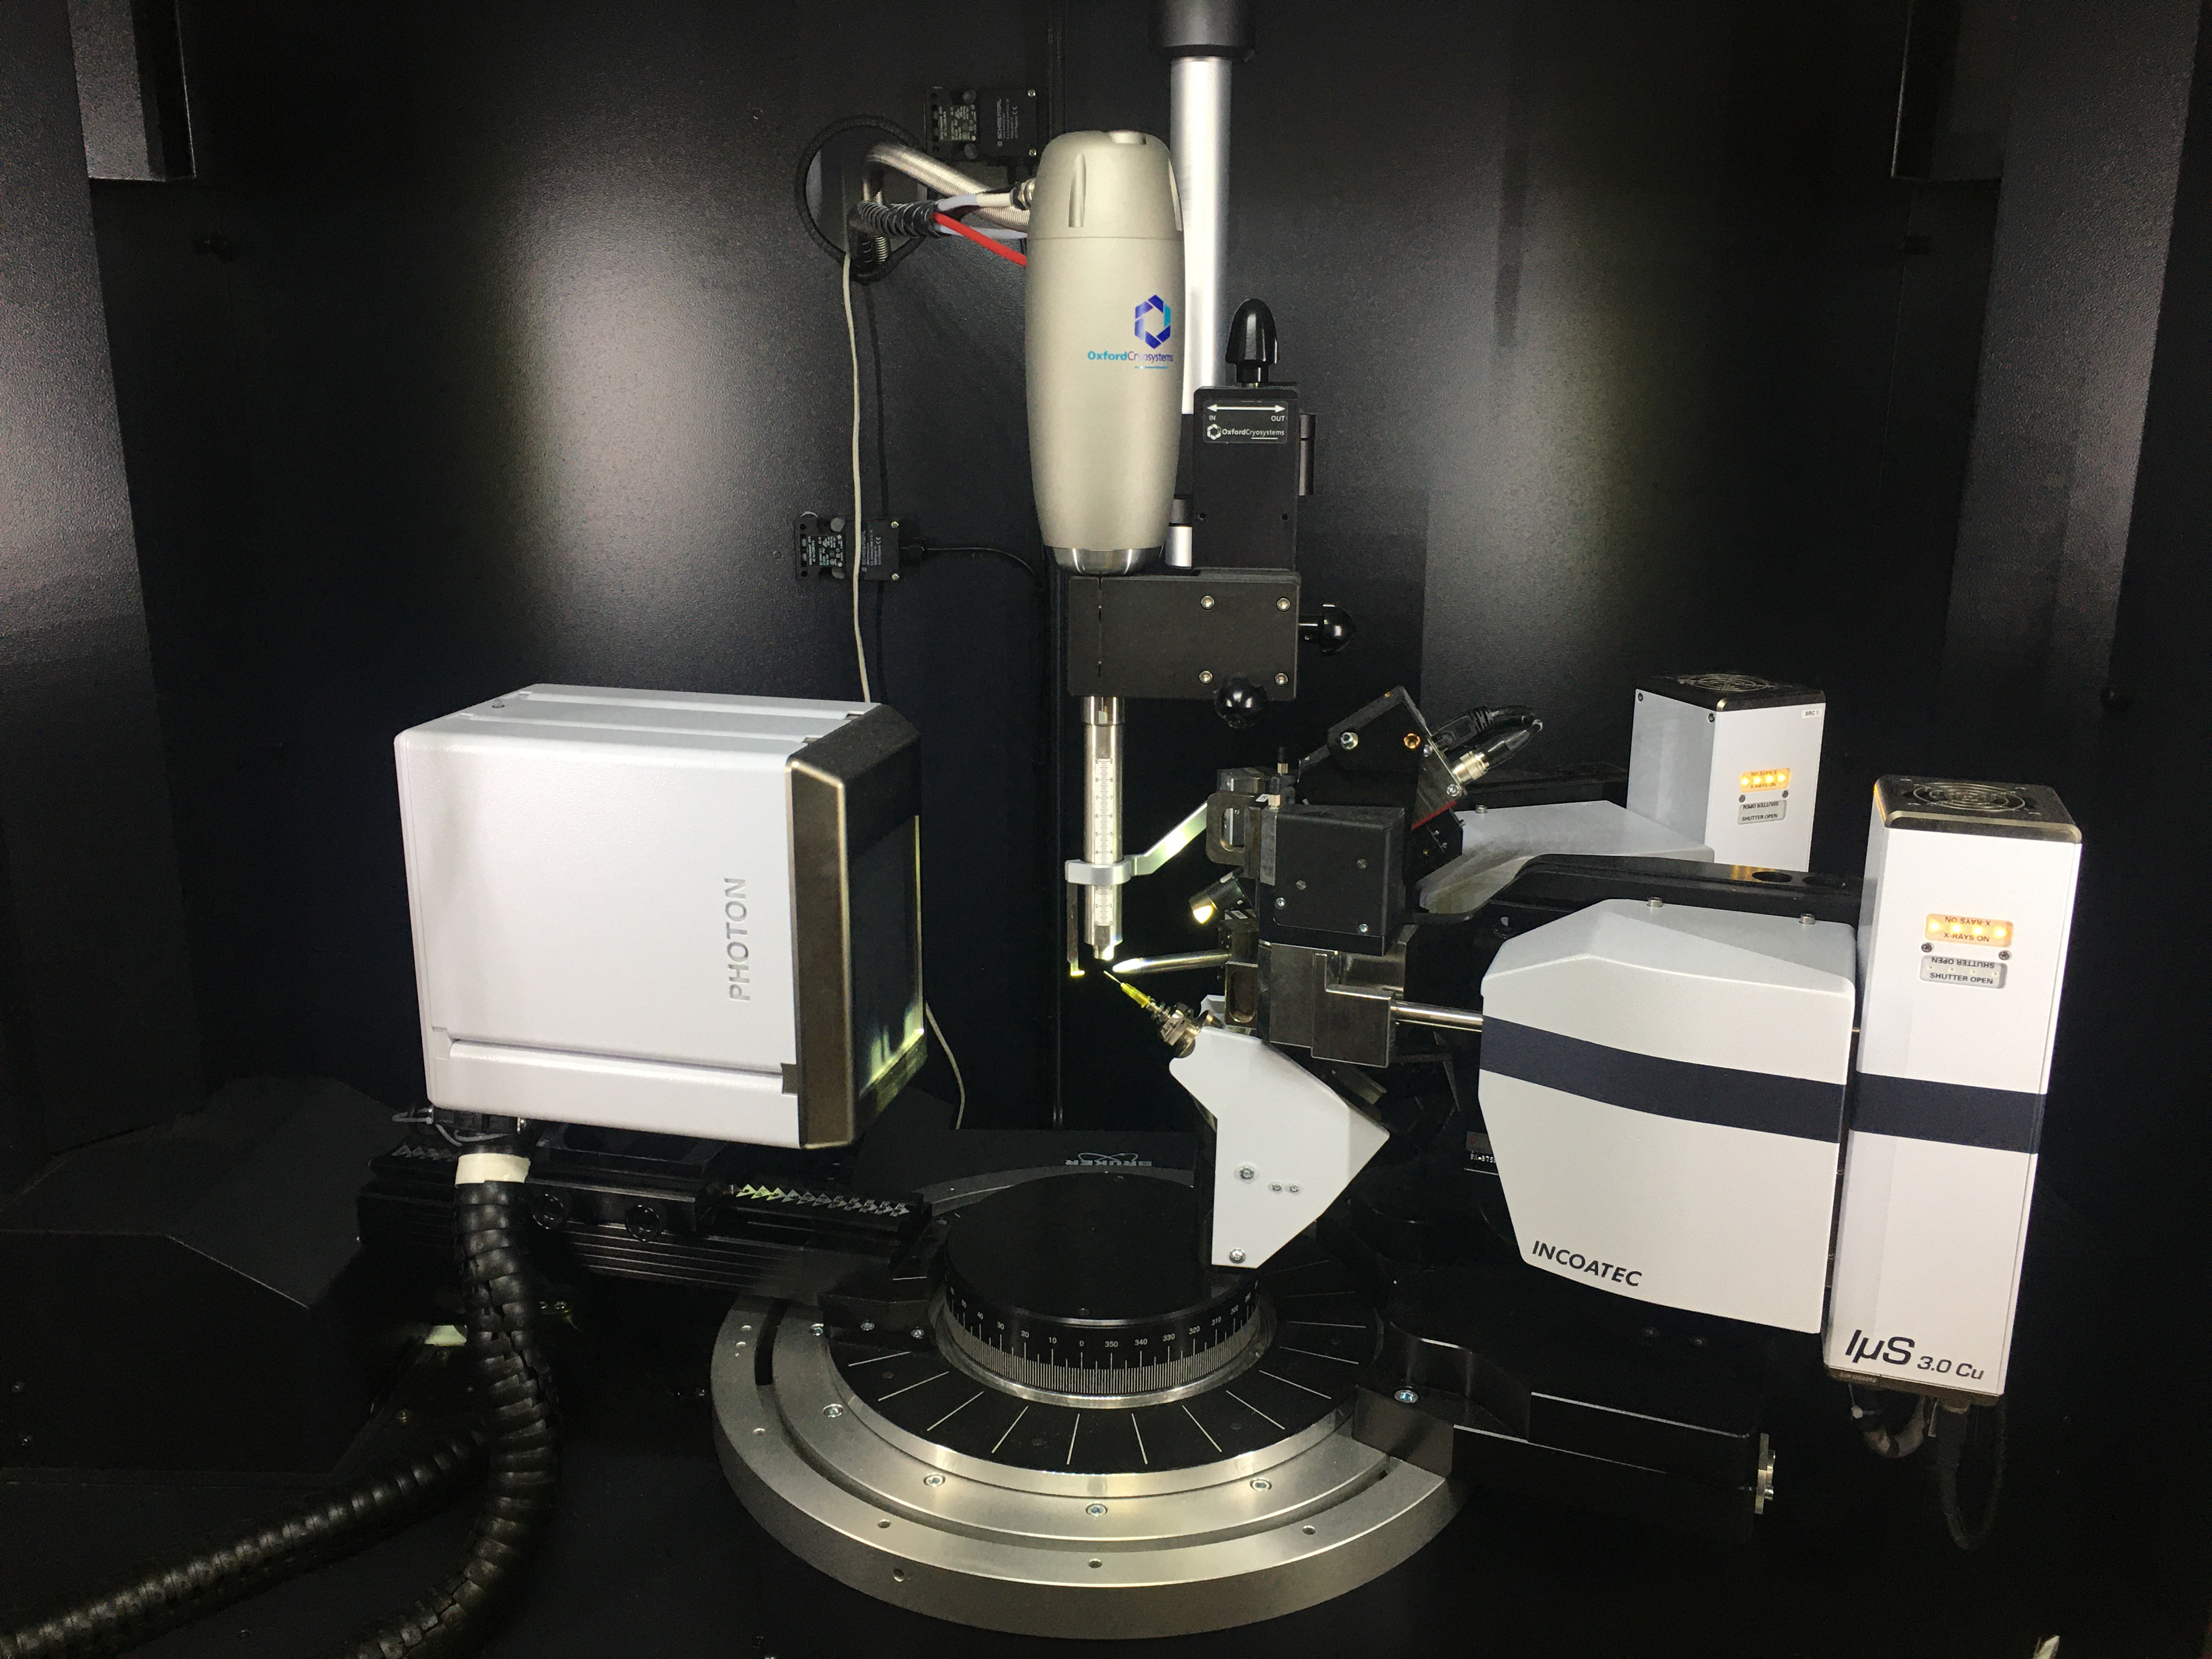
\includegraphics[width=0.8\textwidth]{d8_3.jpeg}
    \caption{Фотография установки}%
    \label{fig:D8_photo}
\end{figure}

\subsection{Исследуемые образцы}

Все изученные монокристаллы имели линейные размеры $\approx50\unit{мкм}$.
Монокристалл Si являлся осколком кристалла, который ранее был исследован на однокристальном спектрометре: $a_\text{Si} = 5.430933 (12)\unit{\AA}$~\cite{Lisoivan:1982}.
Однако, надо учесть, что это значение было вычислено исходя из $\lambda \text{Cu} K\alpha_1 = 1.540562\unit{\AA}$.
При использовании рекомендованной в настоящее время длины волны $\lambda \text{Cu} K\alpha_1 = 1.5405929\unit{\AA}$~\cite{Holzer:1997}, $a_\text{Si} = 5.431042(12)\unit{\AA}$.
Кристалл был смонтирован на гониометрической головке и тщательно сцентрирован (с поворотами по $\omega$ на $\pm 90\degree$). Для определения ориентации кристалла были проведены съемки трех серий $\varphi$-сканов шириной $0.5\degree$ при положениях детектора $2\theta_D = 0, \pm 45\degree$ (D = 70~мм).
Обработку фреймов проводили средствами APEX3 (процедуры: harvest, indexing, refinement), в результате был получен р4р-файл, содержащий информацию об ориентации кристалла относительно осей гониометра.
Аналогичная процедура была проведена с монокристаллом Ge.
Его ПЭЯ уточняли несколько раз методами однокристального спектрометра, многократных отражений и многолучевой дифракции: сводка данных приведена в~\cite{Lisoivan:1982}.
Значения $a_\text{Ge}$ лежат в интервале от $5.65776(2)\unit{\AA}$ до $5.657837(15)\unit{\AA}$, среднее значение $5.65779\unit{\AA}$ наиболее близко к $5.657772(10)\unit{\AA}$ [22].
Пересчет с использованием рекомендованного значения $\lambda \text{Cu} K\alpha_1 = 1.5405929\unit{\AA}$ приводит к $a_\text{Ge} = 5.657885\unit{\AA}$.

Монокристаллы \YEu{} получены методом роста из раствор-рас\-плава.
Продукт синтеза представлял собой мелкокристаллический порошок с размерами кристаллов от 0.2 до 1~мм.
Для исследования было отобрано 5 кристаллов с линейными размерами 20--40~мкм.

\subsection{Измерения в схеме Бонда}

Принципиальная схема эксперимента проведенного в схеме Бонда представлена на рис.~\ref{fig:bond}б.
В нашем случае наличие второго источника рентгеновского излучения ограничивает область доступных углов $2\theta_D$ значениями $\pm 97.5\degree$ (для $D = 128.5\unit{мм}$).
Второе ограничение связано со значительными геометрическими размерами детектора, что не дает блоку с установленной гониометрической головкой размещаться в определенных угловых интервалах.
По полученным р4р-файлам вычисляли углы $\varphi$ и $\omega$ для выведения рефлексов в отражающее положение на экваториальную плоскость.
Съемку рефлексов проводили в режиме $\omega$-сканирования угловых интервалов $\pm 2\degree$ относительно вычисленных значений $\omega$.
Такой интервал позволял зарегистрировать дублет полностью.
При съемке детектор устанавливали под углом $2\theta_D \approx 2\theta_{hkl}$, что обеспечивало регистрацию выбранного рефлекса центральной областью детектора.
Подробно методика описана в~\cite{Kudryavtsev:2024:YEu}.
Методику можно разделить на несколько этапов.

На первом этапе определяли ориентацию монокристалла относительно осей гониометра.
Такая съемка позволяет зарегистрировать существенную часть обратного пространства и провести качественное уточнение элементов матрицы ориентации для последующего вывода выбираемых рефлексов точно в отражающее положение на экваториальную окружность гониометра.
Кроме того, захват области дальних углов необходим для определения условий разрешения дублета $K\alpha$ и выяснения возможности уточнения ПЭЯ.
Обработку полученной серии фреймов проводили по программе APEX3.
В результате определяли предварительные значения ПЭЯ, дифракционный класс и ориентацию кристалла относительно осей гониометра (р4р-файл).
Этот этап соответствует первому этапу проведения РСтА.

Цель второго этапа --- поиск рефлексов, подходящих для измерения $d_{hkl}$.
В первую очередь мы рассматривали рефлексы с угловыми положениями $2\theta$ в узком интервале $\range{95\degree}{98\degree}$.
В случае эталонных монокристаллов (Si и Ge) структура известна, поэтому подходящие рефлексы были выбраны по теоретической дифрактограмме.
В общем случае, т.е. при неизвестной структуре, можно ориентироваться на предварительные значения ПЭЯ и дифракционный класс, установленный на первом этапе.
В случае Si и Ge для измерения ПЭЯ достаточно одного рефлекса, но для оценки уровня случайных ошибок взято большее количество.
Для поиска индексов кристаллографических плоскостей \hkl(h k l), которые могут быть выведены в отражающие положения при двух углах поворота детектора $2\theta_D$, была написана оригинальная программа James (язык Julia), доступная по ссылке https://github.com/m410y/James.jl.
Программа James использует информацию о текущей ориентации кристалла (р4р-файл) и вычисляет углы съемки $\varphi$ и $\omega$, при этом учитывая, что для записи рефлекса необходимо провести $\omega$-сканирование интервала $3-4\degree$.
Кроме этого, учитывается, что вывод в отражающее положение кристаллографической плоскости $(h k l)$, возможен при двух значениях $\omega$, число возможных ориентаций увеличивается вдвое (см. последний столбец табл. 1 Приложения).
Дополнительно программа сигнализирует о случаях, когда может быть использована и фриделевская пара \hkl(-h -k -l).
Съемка фриделевской пары позволяет по разнице значений координат $Y$ максимумов контролировать точность выведения рефлексов на экваториальную плоскость.
Некоторые дополнительные возможности программы James будут описаны далее.

На третьем этапе определяли общие условия проведения $\omega$-сканирования.
Для уменьшения ошибок, связанных с наклонами детектора, положение детектора задавали как $2\theta_D \approx 2\theta_{hkl}$.
При таком положении рефлекс фиксируется центральной областью детектора.
При выборе времени экспозиции ориентировались на получение интенсивности $K\alpha_1$-составляющей в максимуме $2 \cdot 10^4$ импульсов над фоном.
Время накопления фрейма в программе управления Bruker D8 Venture ограничено 10~мин, поэтому при необходимости, для достижения нужного уровня интенсивности, проводили несколько повторных съемок и далее суммировали фреймы средствами программы James. 
На четвертом этапе определяли координаты максимумов средствами программ Origin и James. Установлено, что результаты не отличаются.
Далее вычисляли разницу координат $X$ для двух симметричных положений детектора.
При переходе к углам дифракции рассчитывали угловые размеры пикселя $\gamma$, исходя из физических размеров пикселя ($135.3\unit{мкм}$) и выбранного $D$.
Контроль корректности такого расчета проводили по положениям $K\alpha_{1,2}$ составляющих согласно~\cite{Gromilov:2022}. 
Значение $2\theta_{hkl}$ вычисляли по формуле:
\begin{equation}\label{eq:bond2}
    2\theta_{hkl} = 2\theta_D + \gamma (X_- - X_+) / 2.
\end{equation}
При переходе к межплоскостному расстоянию $d$ использовали эталонное значение длины волны $\lambda \text{Cu} K\alpha_1 = 0.70931715(41)\unit{\AA}$.
Параметр элементарной кубической ячейки вычисляли по известной квадратичной форме: $1/d^2 = (h^2 + k^2 +l^2)/a^2$.

\section{Изучение эталонных кристаллов Si и Ge}

Для измерения ПЭЯ Si, с учетом ранее обозначенных приборных ограничений, наиболее подходят три семейства кристаллографических плоскостей \hkl{11 3 1}, \hkl{9 7 1} и \hkl{9 5 5} c $2\theta = 96.737\degree$.
В случае Ge выбраны семейства \hkl{10 6 0} и \hkl{8 6 6} с $2\theta = 93.949\degree$.
Поиск подходящих рефлексов средствами программы APEX3 можно сделать только в ручном режиме, т.е. последовательно прелагая значения \hkl(h k l).
Возможны два варианта расчетов: первый предполагает определение углов для вывода кристаллографического направления навстречу пучку ($\varphi_0$ и $\omega_0$), второй --- углов для установки кристаллографической плоскости в отражающее положение при положении детектора в отрицательных углах $2\theta_D$.
В обоих вариантах предлагается только одно значение $\varphi$ (из двух возможных).
Такого функционала совершенно недостаточно для учета эксцентриситета образца: согласно~\cite{Ponomarev:1969} необходимо подобрать пару рефлексов \hkl(h k l), которые можно зафиксировать при положениях гониостата $\omega \approx \pm 90\degree$ (см. рис.~\ref{fig:eccentr}).
В случае Si, число симметрично связанных плоскостей равно 120 (для Ge –-- 48) и сделать это средствами программы APEX3 проблематично.
Необходимые расчеты были проведены по программе James.

\begin{figure}[ht!]
    \centering
    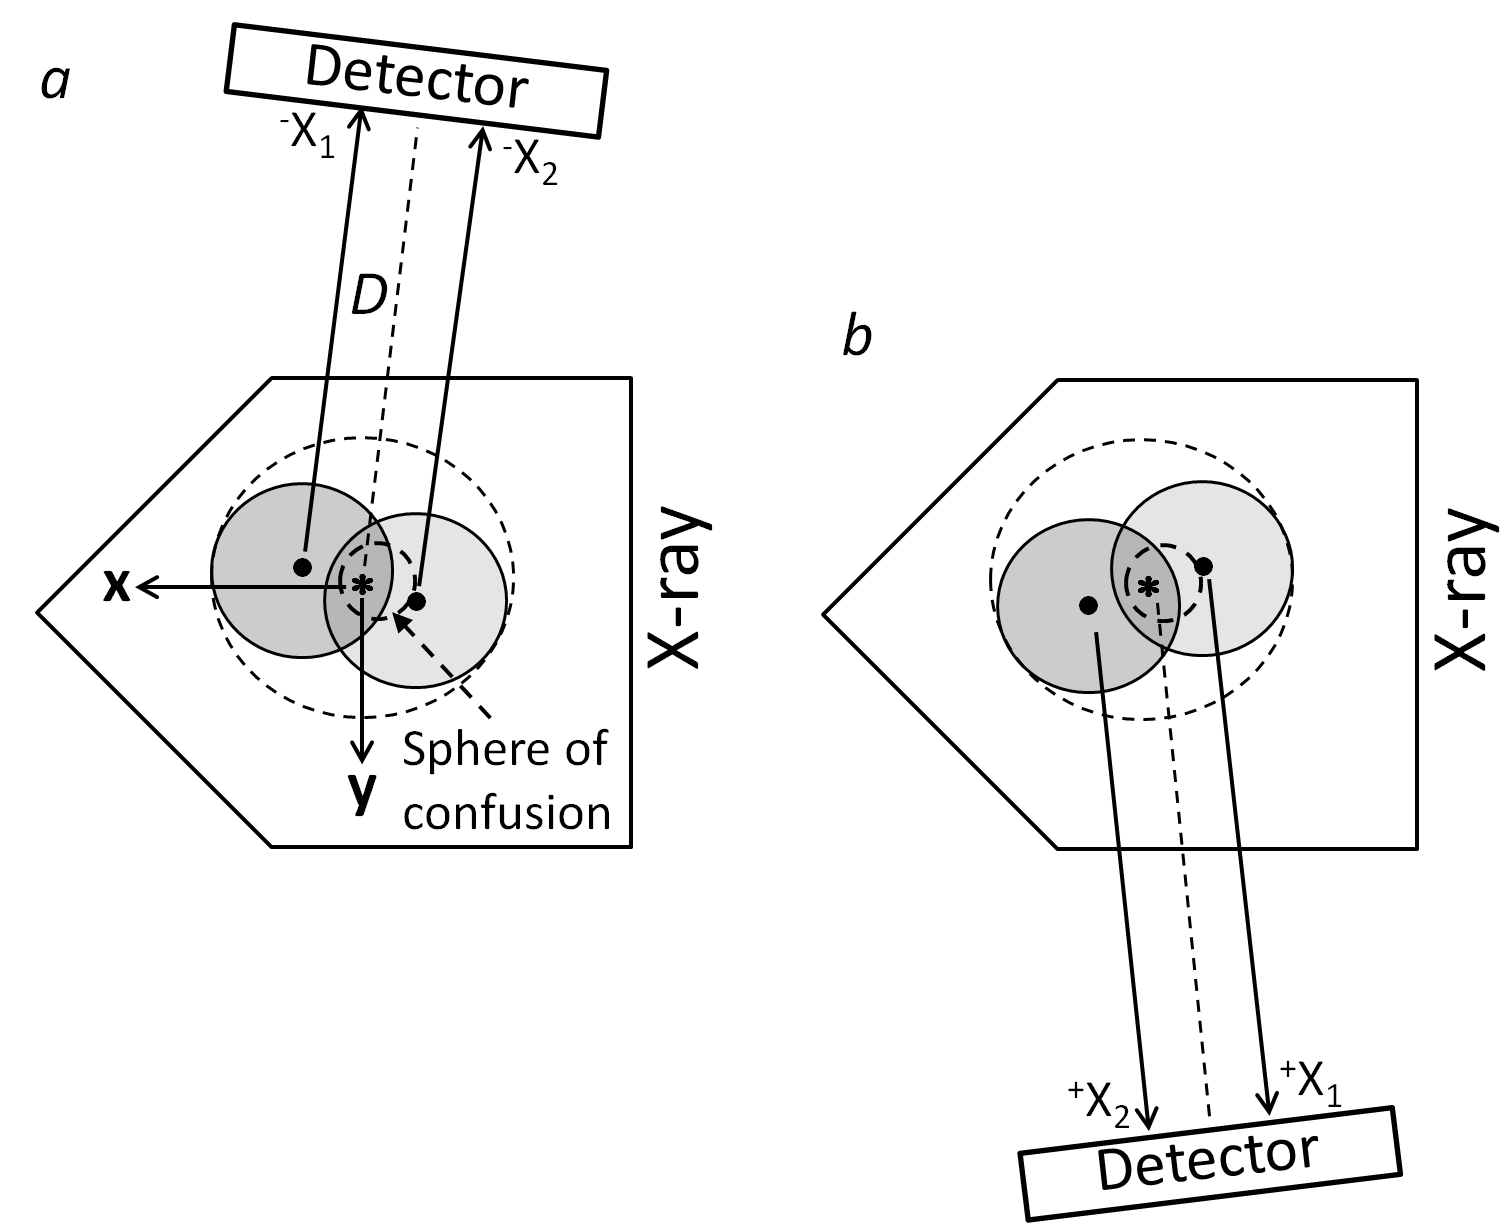
\includegraphics[width=0.8\textwidth]{eccentr.png}
    \caption{Схемы эксперимента для учета эксцентриситета образца}%
    \label{fig:eccentr}
\end{figure}

Первая часть программы James позволяет находить среди множества плоскостей, связанных симметрией такие, которые можно вывести в отражающее положение хотя бы при одном (из двух симметричных) положении детектора.
Для этого используется информация о текущей ориентации кристалла на гониометре, т.е. p4p-файл, в котором находится матрица ориентации UB~\cite{Busing:1967} и предварительные значения ПЭЯ.
Углы гониометра $\varphi$ и $\omega$, необходимые для выведения каждой плоскости в отражающее положение на экваториальную плоскость, вычисляются исходя из известной длины волны, размеров пикселя, расстояния до детектора и других неизменных параметров прибора.
В каждом случае проверяются геометрические ограничения прибора.
Полученная информация для всех подходящих рефлексов собирается в таблицу Excel, ее можно проанализировать и провести отбор.

Вторая часть программы James связана с обработкой полученных фреймов, т.е. описанием 2D-профиля дублета. На входе она использует p4p-файл и информацию о примерном положении центра детектора (результат юстировки, прямое определение, калибровка).
Из экспериментального фрейма вырезается центральная область ($X = \pm 30\unit{пикс.}$, $Y = \pm 15\unit{пикс.}$), в которой, исходя из $2\theta_D \approx 2\theta_{hkl}$, должен находиться искомый рефлекс.
Медианное значение интенсивности принимается за начальное значение фона.
Пиксели с интенсивностью больше заранее заданной принимаются за ''горячие пиксели'' и их значения приравниваются среднему значению по 8 соседним пикселям.
После учета горячих пикселей максимум интенсивности в выбранной области назначается примерным положением $K\alpha_1$-составляющей.
Далее, исходя из значений $D$ и $2\theta$ рассчитывается положение $K\alpha_2$-составляющей и обе точки смещаются так, чтобы теоретическое положение $K\alpha_1$ совпадало с координатами найденного максимума интенсивности.
Аппроксимация дублета проводится двумя независимыми  функциями 2D-Gauss, т.е. без закрепления междублетного расстояния и соотношения интенсивностей составляющих $2/1$.
Направлениями главных осей берутся вдоль координат детектора $X$ и $Y$ детектора.
В наших экспериментах именно функция 2D-Gauss наиболее хорошо описывала форму пика при минимальном числе уточняемых параметров: координаты максимума, полуширины (ширина на половине высоты, FWHM) в направлениях $X$ и $Y$, и интегральная интенсивность.

\subsection{Оценка и учет эксцентриситета образца Si}

Несмотря на тщательную центрировку образца (в том числе с контрольными разворотами по оси $\omega$) крайне сложно точно определить центр образца, особенно при его неопределенной форме.
Можно ожидать, что при повороте вокруг оси $\omega$ центр образца движется по окружности, а сам образец описывает торообразную поверхность, ее условный внешний контур показан на рис.~\ref{fig:eccentr} штриховой окружностью.
Выход оси $\omega$ показан звездочкой: считаем, что в общем случае ось не пересекается центром первичного пучка.
Подобную картину можно ожидать и при повороте образца вокруг оси $\varphi$.
Так как для использованного гониометра паспортное значение диаметра сферы сведения осей (sphere of confusion) составляет 7~мкм, центр образца при повороте вокруг обеих осей движется по достаточно сложной траектории.

Для оценки смещений центра образца при повороте вокруг оси $\varphi$, среди доступных для измерения рефлексов от семейств кристаллографических плоскостей типа \hkl{11 3 1}, \hkl{9 7 1} и \hkl{9 5 5}, было выбрано 10 вариантов, у которых значения $\omega$ лежат в интервале от $-82\degree$ до $-95\degree$.
Это примерно соответствует позиции образца при центрировании.
Все съемки проведены при положении детектора: $2\theta_D = -96.7\degree$, $D = 128.53\unit{мм}$.
Зависимость $X(\varphi)$ представлена на рис.~\ref{fig:eccentrSi}а.
Интервал значений $X$ составляет $\approx 0.3$~пикселя, что с учетом размера пикселя, соответствует смещениям центра образца с оси $\varphi$ на 20~мкм.

\begin{figure}[ht!]
    \centering
    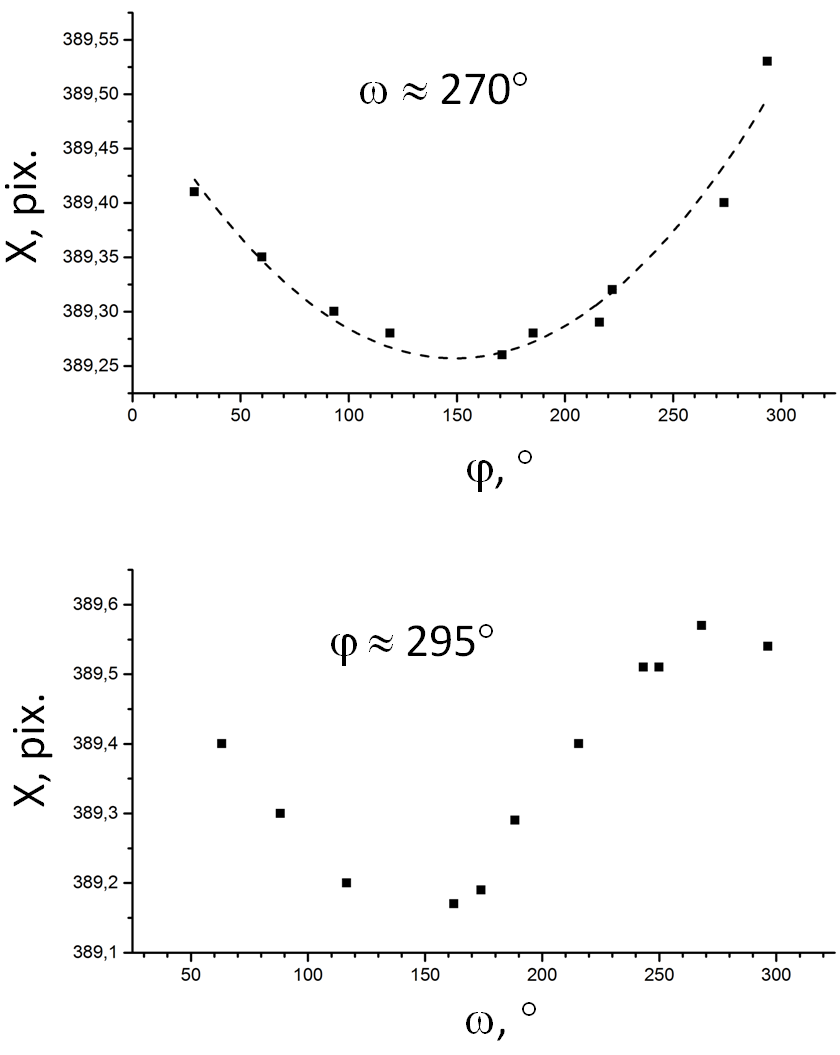
\includegraphics[width=0.8\textwidth]{eccentrSi.png}
    \caption{Смещение максимумов дифракционных отражений из-за эксцентриситета образца}%
    \label{fig:eccentrSi}
\end{figure}

Таким образом, два проведенных эксперимента показали одинаковые картины эксцентриситетов, связанных с поворотами образца вокруг осей $\omega$ и $\varphi$.
При измерении ПЭЯ наиболее разумно исключить влияние именно последнего, тогда далее можно использовать подход, предложенный в~\cite{Ponomarev:1969}.
Он заключается в съемке фриделевской пары со значениями $\omega \approx \pm 90\degree$, что соответствует крайним положениям центра образца в направлении первичного пучка.
На рис.~\ref{fig:eccentr} центры образцов показаны жирными точками.
Очевидно, что при таких положениях образца можно ожидать максимальных смещений дифракционных рефлексов.
Среди всех вариантов, предложенных программой James, были выделены 5 фриделевских пар, удовлетворяющих этому критерию.
Их индексы и установочные углы $\varphi$ и $\omega$ представлены в табл.~\ref{tab:Si} Приложения.
Там же даны координаты максимумов рефлексов, зарегистрированных при симметричных положениях детектора $2\theta_D = 96.7\degree$ и средние значения для каждой пары $\left<X\right> = (X_1 + X_2) / 2$.
Как следует из рис.~\ref{fig:eccentr} значения $\left<X\right>$ соответствует мнимому положению кристалла на оси вращения $\omega$.
Для учета эксцентриситета в формуле~(\ref{eq:bond2}) вместо значений $X$ необходимо использовать значения $\left<X\right>$.
Чтобы различать рефлексы, зарегистрированные при симметричных положениях детектора, введем надстрочные индексы <<$-$>> и <<$+$>>, тогда выражение~\ref{eq:bond2} можно представить в следующем виде:
\begin{equation}\label{eq:bond4}
    2\theta_{hkl} = 2\theta_D + \gamma (X_1^- + X_2^- - X_1^+ - X_2^+) / 4 = 2\theta_D + \gamma (\left<X\right>^- - \left<X\right>^+) / 2
\end{equation}
где $\gamma$ --- угловой размер пикселя.

\subsection{Определение угловых размеров пикселя}

При регистрации рефлекса центральной областью детектора (как в нашем случае) значение $\gamma$ можно вычислить исходя из физических размеров пикселя $P$ (в нашем случае 0.1353~мм) и расстояния от образца до детектора $D$ (в нашем случае 128.53~мм) по формуле:
\begin{equation}\label{eq:pixsize}
    \gamma = \frac{P}{D}
\end{equation}
Однако значение $D$, которое показывает прибор, всегда можно поставить под сомнение.
Правильнее провести калибровку положения детектора, например, согласно методике~\cite{Panchenko:2023}.
Для этого съемка эталонного монокристалла Si была проведена путем $\omega$-сканирования интервалов $10\degree$ в области углов $200\degree$ при пяти положениях кристалла по углу $\varphi$ (шаг $10\degree$).
Обработка полученных фреймов проведена по программе SearchXY~\cite{Panchenko:2023}.
В результате получено значение $D = 128.21\unit{мм}$.
Развороты детектора (rot1, rot2, rot3) в наших экспериментах можно не учитывать, т.к. регистрация рефлексов проводится центральной областью детектора.
Итоговое значение $\gamma = 0.06033\degree$.

Не всегда проведение полной калибровки положения детектора целесообразно, т.к. она занимает достаточно много времени.
Можно согласно~\cite{Gromilov:2022} использовать данные о положении $K\alpha_1$- и $K\alpha_2$-составляющих любого из изученных рефлексов эталона, тогда по разнице значений $X$ и теоретическим положениям углов $2\theta$  $K\alpha_{1,2}$-составляющих значение $\gamma$ вычисляют по формуле:
\begin{equation}\label{eq:pixsize_exp}
    \gamma = \frac{2\theta_2 - 2\theta_1}{\Delta X}
\end{equation}

Другой подход к определению $\gamma$ основан на съемке одного и того же рефлекса при двух угловых положениях детектора.
Так, рефлекс \hkl(-11 1 -3) Si был отснят при $2\theta_A = 96.4\degree$ и $2\theta_B = 97.0\degree$.
Смещение максимума $\Delta X$ позволяет провести вычисление $\gamma$ по формуле:
\begin{equation}\label{eq:pixsize_exp_2}
    \gamma = \frac{2\theta_A - 2\theta_B}{\Delta X} = 0.06033\degree
\end{equation}

Отметим, что такой подход позволяет проводить измерения при минимальных отклонениях рефлекса от центра детектора.
Полученное значение идеально совпадает с результатом, полученным по результатам полной калибровки.

\subsection{Вычисление ПЭЯ Si}

Полученное значение $\gamma$ позволяет вычислить $a_\text{Si}$.
При произвольном выборе рефлексов из табл.~\ref{tab:Si} Приложения расчет согласно~\ref{eq:bond2} приводит к значениям угла $2\theta$ в интервале $\range{96.722\degree}{96.747\degree}$: отклонения от теоретического значения $96.734\degree$ достигают $0.013\degree$.
Учет эксцентриситета согласно~\ref{eq:bond4} с использованием произвольных пар средних значений $\left<X\right>^-$ и $\left<X\right>^+$ уменьшает интервал значений $2\theta$ до $\range{96.730\degree}{96.736\degree}$ а отклонения от теоретического значения не превышают $0.004\degree$.
Использование рефлексов с близкими значениями углов $\varphi = -66.31\degree$ и $59.35\degree$ (индексы рефлексов выделены в табл.~\ref{tab:Si} Приложения жирным) позволяет учесть эксцентриситет, связанный с поворотом образца вокруг оси $\varphi$.
Конечные результаты уточнения: $2\theta = 96.732\degree$, $d = 0.47452 (3)\unit{\AA}$, $\Delta d / d = 6.2 \cdot 10^{-5}$, $a = 5.4311(3)\unit{\AA}$ (в скобках указаны абсолютные погрешности, вычисленные для $\Delta 2 \theta = 0.004\degree$).
Можно отметить, что полученное значение $a_\text{Si}$ отклоняется от эталонного всего на $0.00006\unit{\AA}$.
Чтобы полностью исключить влияние эксцентриситета, связанного с поворотом кристалла вокруг оси $\varphi$, необходимо вывести одно из кристаллографических направлений вдоль оси $\omega$, тогда измерения можно проводить на рефлексах типа \hkl{h k 0}.
При использовании гониометра с изменяемым углом $\chi$ (т.е. четырехкружного) такая проблема не возникает.
В нашем случае угол $\chi$ на гониометре фиксирован, а штатные гониометрические головки предполагают только линейные перемещения образца.

\subsection{Вычисление ПЭЯ Ge}

Для устранения эксцентриситета, связанного с поворотом кристалла вокруг оси $\varphi$ монокристалл Ge был смонтирован на оригинальной гониометрической головке, имеющей возможность поворота образца вокруг одной оси на $\pm 10\degree$ (далее гониометрическая $\chi$-головка).
После определения ориентации кристалла, с помощью программы James были рассчитаны углы для выведения кристаллографического направления вдоль оси $\omega$, для этого был использован следующий алгоритм.

Повороты образца описываются эйлеровыми углами $\varphi$, $\omega$ и $\chi$.
Правосторонняя декартова система координат гониометра задана следующим образом.
Направление оси $x$ совпадает с направлением первичного пучка.
Если смотреть навстречу $x$, то положительным изменением угла $\omega$ будет вращение против часовой стрелки.
Ось $z$ выбирается в направлении оси $\omega$ и против направления оси $\varphi$ (в нулевом положении для четырехкружного гониометра).
Направление оси $y$ задается автоматически.
Ось $\chi$ направлена против оси $x$, в нашем случае соответствующий ей угол поворота фиксирован и равен приблизительно $55\degree$.

Нулевой угол дуги нашей гониометрической головки обозначим $\chi^\ast$.
Т.к. кристаллографическое направление можно вывести вдоль или против $z$, то число возможных вариантов $\chi$ и $\chi^\ast$ может быть равно 4 (2 в вырожденном случае) или 0 (если процедура невозможна).
Ограничение значений угла $\chi^\ast$ связано с диапазоном углов дуги гониометрической головки, в нашем случае $\pm 10\degree$.

Если задать кристаллографическое направление \hkl[h k l] в виде трехмерного вектора $s$, получающегося домножением вектора-столбца \hkl(h k l) на матрицу ориентации UB, то определить возможность выведения рефлекса можно по углу $\theta_s$ между $s$ и $x$ и полярному углу $\varphi$ проекции $s$ на плоскость $yz$ (рис.~\ref{fig:scheme}).
Кристаллографическое направление можно вывести вдоль оси $\omega$ если $\sin{\theta_s} > \cos{\chi}$.
В этом случае углы $\chi^\ast$ будут равны:
\[ \varphi_s - \arcsin\left(\frac{\cos{\chi}}{\sin{\theta_s}}\right) \]
\[ \varphi_s + \arcsin\left(\frac{\cos{\chi}}{\sin{\theta_s}}\right) + 180\degree \]
\[ \varphi_s + \arcsin\left(\frac{\cos{\chi}}{\sin{\theta_s}}\right) \]
\[ \varphi_s - \arcsin\left(\frac{\cos{\chi}}{\sin{\theta_s}}\right) + 180\degree \]

При значении $\cos{\chi} > 0$ первые два угла соответствуют выведению $s$ вдоль $x$, а другие --- $-x$. При смене знака $\cos{\chi}$ картина меняется на противоположную.
Соответствующие углы $\omega$ будут равны:
\[\arctan\left(-\sqrt{\sin^2{\theta_s} - \cos^2{\chi}}, -\cos{\theta_s}\right)\]
\[\arctan\left(\sqrt{\sin^2{\theta_s} - \cos^2{\chi}}, -\cos{\theta_s}\right)\]
\[\arctan\left(\sqrt{\sin^2{\theta_s} - \cos^2{\chi}}, \cos{\theta_s}\right)\]
\[\arctan\left(-\sqrt{\sin^2{\theta_s} - \cos^2{\chi}}, \cos{\theta_s}\right)\]

где $\arctan(y, x)$ –-- полярный угол точки с координатами $(x, y)$ на координатной плоскости. 

\begin{figure}[ht!]
    \centering
    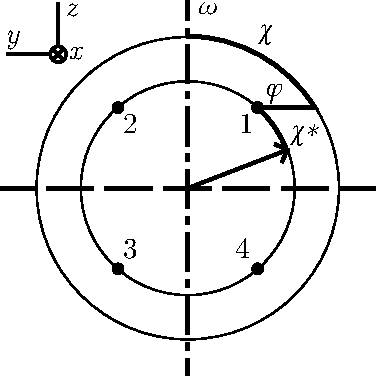
\includegraphics{scheme.pdf}
    \caption{Схема направления осей гониометра}%
    \label{fig:scheme}
\end{figure}

Расчеты для монокристалла Ge показали, что вдоль оси $\omega$ можно вывести направление \hkl{0 1 0}, т.к. для него значение угла $\chi^\ast = 2.2\degree$.
После соответствующего поворота образца на гониометрической $\chi$-головке, исследование в схеме Бонда было проведено по рефлексам типа \hkl{10 0 6} (теоретическое значение $2\theta = 93.943\degree$).
Все рефлексы регистрировали при одинаковых значениях угла $\varphi = -179.06\degree$.
Приборные ограничения позволили отснять только 12 из 16 теоретически возможных рефлексов, координаты их максимумов приведены в табл.~\ref{tab:Ge} Приложения.
При произвольных сочетаниях рефлексов, возможны 36 вариантов пар, тогда значения $2\theta$, вычисленные согласно~\ref{eq:bond2}, лежат в интервале $\range{93.935\degree}{93.958\degree}$.
Максимальные отклонения от теоретического значения достигают $0.015\degree$.
Для учета эксцентриситета согласно~\ref{eq:bond4} были использованы 4 пары значений $\left<X\right>$, при этом вычисленные значения $2\theta$ укладываются в узкий интервал $\range{93.943\degree}{93.945\degree}$, а отклонения от теоретического значения не превышают $0.001\degree$.
Если использовать среднее значение $2\theta = 93.945\degree$, то: $d = 0.48515 (3)\unit{\AA}$, $\Delta d / d = 6.5 \cdot 10^{-5}$, $a = 5.6578 (4)\unit{\AA}$.
Отклонение полученного $a_\text{Ge}$ от теоретического значения $5.657885\unit{\AA}$ составляет 
$0.0001\unit{\AA}$.

Анализ координат $Y$ рефлексов Ge (см. табл.~\ref{tab:Ge} Приложения) позволяет оценить точность выведения направления $b$ вдоль оси $\omega$.
Для этого можно построить зависимости $Y$ от $\omega$ для экспериментов, проведенных при двух симметричных положениях детектора $2\theta_D = 93.9\degree$.
В обоих случаях зависимости хорошо описываются синусоидами, но при $2\theta_D = -93.9\degree$ фаза сдвигается на $\theta$, а при $2\theta_D = +93.9\degree$ на $\theta + 180\degree$.
Для одновременной обработки всех рефлексов значения сдвигов вычитали из первичных значений $\omega$.
Из построенной аппроксимации (см. рис.~\ref{fig:eccentrGe}) следует, что максимальная разница значений $Y$ составляет $\approx 2.2\unit{пикс.}$, что соответствует отклонению направления $b$ от оси $\omega$ $0.13\degree$.
Такой показатель соответствует цене нониусной шкале дуги использованной гониометрической головки.
Т.к. отклонение лежит в плоскости дуги гониометрической головки, можно утверждать, что оно связано преимущественно именно с погрешностью установки угла $\chi^\ast$, а не угла $\varphi$.

\begin{figure}[ht!]
    \centering
    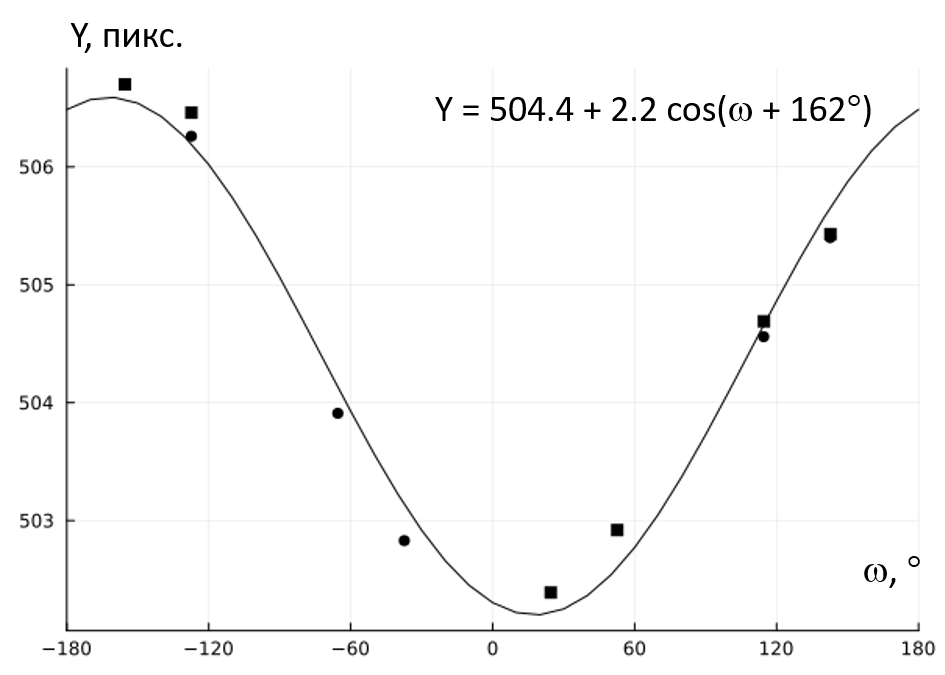
\includegraphics[height=0.5\textwidth]{eccentrGe.png}
    \caption{Зависимость координат $Y$ от угла $\omega$ для монокристалла Ge.}%
    \label{fig:eccentrGe}
\end{figure}

Выведение кристаллографического направления вдоль оси $\omega$ позволяет не только определять межплоскостные расстояния и ПЭЯ, но и углы между кристаллографическими плоскостями типа \hkl[h 0 l].
Так, для изученного монокристалла Ge было проведено измерение угла между плоскостями \hkl[6 0 -10] и \hkl[10 0 -6].
Для этого получена зависимость интенсивности рефлекса от угла $\omega$ с помощью $\omega$-сканирования диапазона $0.4\degree$, содержащего максимум интенсивности рефлекса от $K\alpha_1$ с шагом $0.002\degree$.
Для каждой позиции проводили суммирование интенсивности всех пикселей в прямоугольной области детектора $50\times30$.
Значение угла $\omega$, при котором достигается максимальная интенсивность, было получено аппроксимацией полученной зависимости $I(\omega)$ полиномом второй степени.
В результате, полученные значения углов $\omega$ составили $67.6113 (2)\degree$ и $95.6731 (2)\degree$ для рефлексов \hkl[6 0 -10] и \hkl[10 0 -6] соответственно.
Разница значений составила $28.0618 (4)\degree$, что отличается от идеального значения $28.0725\degree$ на $0.0107 (4)\degree$.

Проведенные эксперименты с эталонными монокристаллами показывают, что учет эксцентриситета образца вокруг оси $\omega$ с ограничением углов $\varphi$ позволяет получать значения углов $2\theta$ с точностью не хуже $0.004\degree$.
Особо отметим, что это не среднее значение по нескольким экспериментам, а максимальное отклонение.
При сохранении такого показателя повышение точности измерений ПЭЯ возможно лишь при увеличении углов $2\theta$.
При использовании дифрактометра, оборудованного 2D-детектором, это можно достичь лишь путем использования рефлексов на краю детектора.
Так, при установке детектора в позиции $D = 128.5\unit{мм}$ и $2\theta_D = 97\degree$ можно регистрировать рефлексы вплоть до $118\degree$, что теоретически должно привести к уменьшению относительной ошибки $\Delta d / d$ вдвое.
Однако, такой путь предполагает проведение двух полных калибровок прибора при симметричных положениях детектора.Гораздо перспективней использовать дополнительный детектор меньших размеров, как это будет описано далее.

Другое ограничение точности измерений связано с большой шириной дифракционных отражений: даже для исследованных эталонных монокристаллов значения FWHM достигают $0.12\degree$, что в первую очередь обусловлено расходимостью первичного пучка.
К недостаткам лабораторных дифрактометров можно отнести и недостаточную светосилу.
В нашем случае, несмотря на использование микрофокусного источника 3-го поколения, измерение одного рефлекса Si составило 2 часа, т.е. съемка 4-х рефлексов для учета эксцентриситета занимала 8 час.
Большое время эксперимента существенно ограничивает эксперименты по изучению динамики изменения ПЭЯ при внешних воздействиях.
Конечно, можно пожертвовать точностью и перейти к исследованию рефлексов с меньшими значениями $2\theta_D$, но большей интенсивностью.
Все указанные недостатки могут быть существенно уменьшены при переходе на синхротронное излучение.
Так на станции 1.2 «Структурная диагностика» ЦКП СКИФ (г. Новосибирск) будет установлен монокристальный дифрактометр.
Даже если он будет оснащен двухкружным гониометром, минимальная дооснастка (гониометрическая $\chi$-головка, дополнительный детектор) позволит проводить прецизионное измерение ПЭЯ с $\Delta d / d \approx 10^{-6}$.
Однако, для измерения параметров элементарной ячейки кристаллов с низкой симметрией (триклинной или моноклинной) предпочтительней использовать четырехкружный гониометр, что позволит избежать нескольких переклеек кристалла.

\section{Изучение однородности монокристаллов \YEu{}}

При выборе рефлекса, подходящего для уточнения ПЭЯ, мы столкнулись с проблемой оценки его интенсивности.
Так, например, теоретические значения $F$ рефлексов \hkl(6 8 20) и \hkl(8 6 20), с одинаковым угловым положением $2\theta$, соотносятся как $\approx 7/1$.
Естественно, предпочтительно использовать наиболее интенсивное отражение.
Для решения этой проблемы предварительная съемка кристалла была скорректирована --- расстояние $D$ уменьшено до $60\unit{мм}$, а углы $2\theta_D$ увеличены до $\pm 75\degree$.
В результате были построены сечения обратного пространства (см. рис.~\ref{fig:precession}), захватывающие область углов $2\theta \range{95\degree}{100\degree}$.
Сопоставление интенсивностей рефлексов с результатами вычислений программы James позволило выбрать оптимальные индексы.
По такой схеме было проведено исследование 5 монокристаллов, результаты представлены в табл. 3. Значения ПЭЯ лежат в интервале от $10.6902\unit{\AA}$ до $10.7045\unit{\AA}$, разница крайних значений составляет $0.0143\unit{\AA}$, что значительно превосходит абсолютную погрешность определения ПЭЯ равную $0.0007\unit{\AA}$.
Таким образом, можно однозначно утверждать, что синтезированный продукт не однороден.

\begin{figure}[ht!]
    \centering
    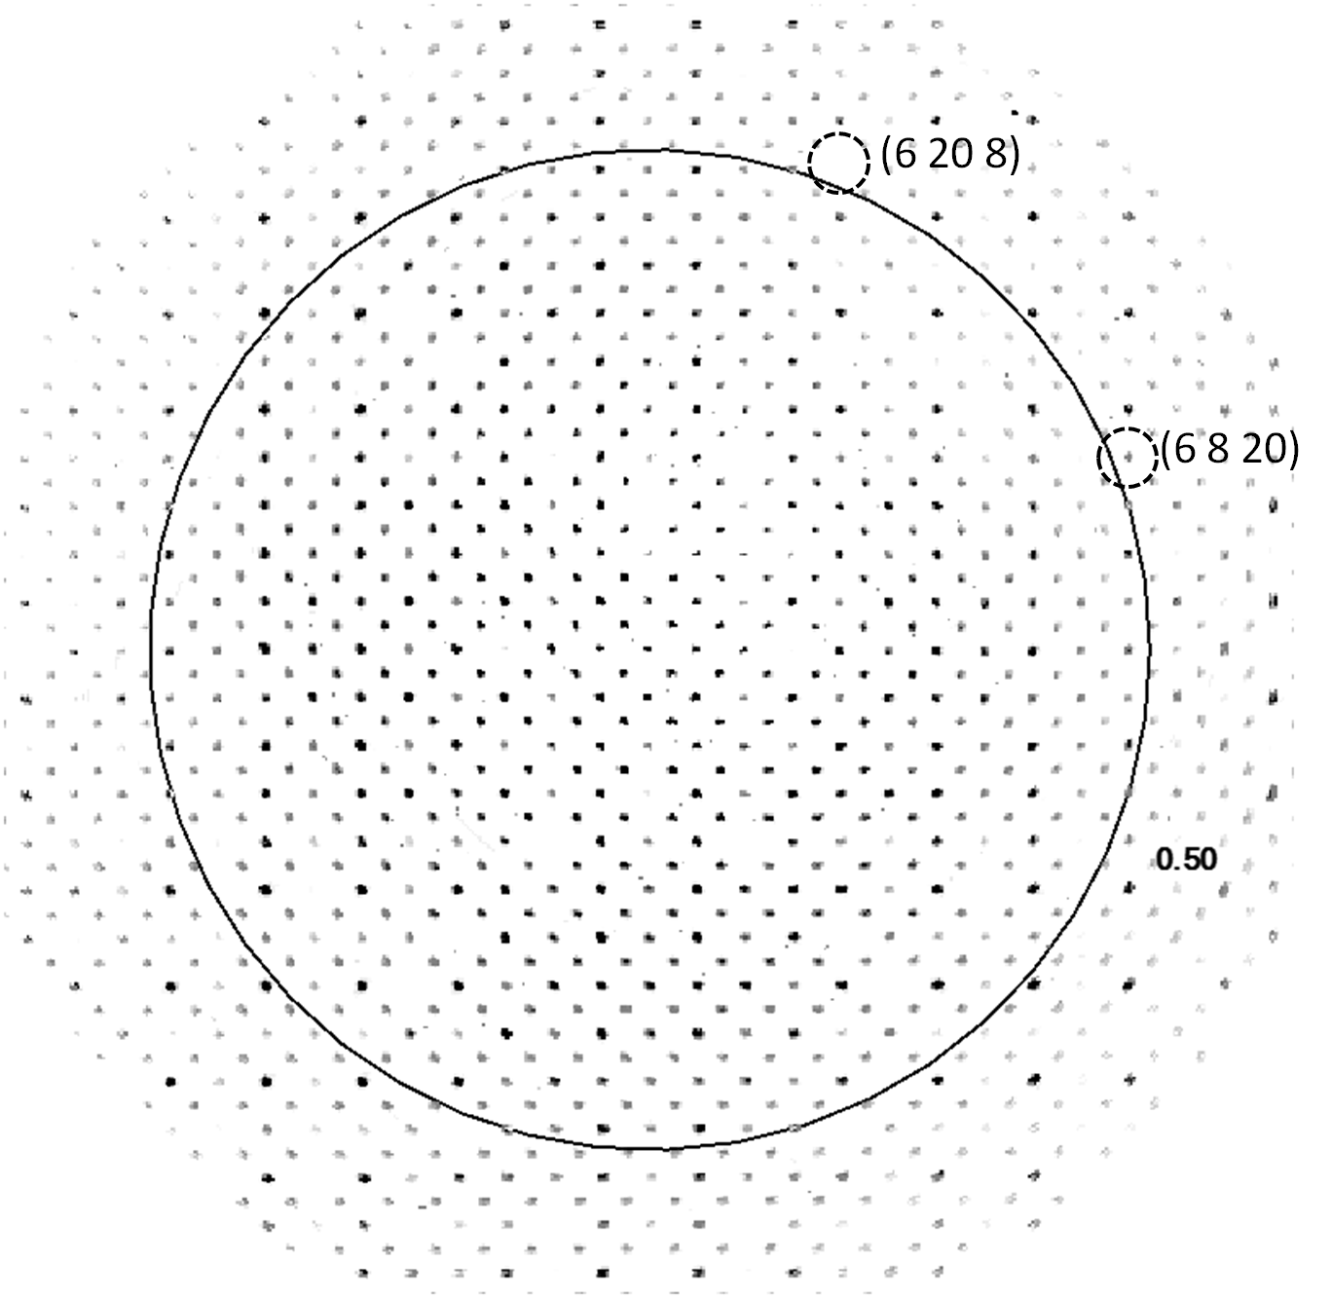
\includegraphics[width=0.8\textwidth]{precession.png}
    \caption{Сечение обратного пространства}%
    \label{fig:precession}
\end{figure}

Для оценки соотношения Y/Eu в изученных монокристаллах можно использовать правило Вегарда.
Для построения соответствующей прямой были использованы литературные данные~\cite{Swanson:1954,Morris:1984,Nikolaev:2023}, а также результаты проведенного нами РСтА 5 кристаллов, отобранных из того же самого продукта синтеза, из которого отобран кристалл $C$ (см. табл. 4 Приложения).
Вместо утерянного кристалла №2 был изучен №6.
Расчет стратегии съемки для накопления полного массива данных производился для каждого кристалла автоматически с учетом его симметрии \hkl(m -3) по предварительно определенной матрице ориентации с использованием пакета программ APEX3.
Далее проводили интегрирование экспериментальных интенсивностей и вводили поправки на поглощение.
Структуры решены с помощью программы ShelxT~\cite{Sheldrick:2015:shelxt} и уточнены с ShelxL~\cite{Sheldrick:2015:shelxl} в графическом интерфейсе Olex2~\cite{Dolomanov:2009}.
Параметры атомных смещений были уточнены в анизотропном приближении.
В результате установлено, что все изученные кристаллы изоструктурны и представляют собой твердые растворы \YEu{}, причем смешанными оказываются обе позиции металла.
Для примера приведем результат исследования кристалла №5: $x = 0.277(10)$, $a = 10.69180(10)\unit{\AA}$, $V = 1222.23(3)\unit{\AA}^3$; пр. гр. $Ia-3$, $Z = 16$, $\rho_\text{выч} = 5.669\unit{г/см}^3$, $\mu_\text{выч} = 38.366\unit{мм}^{-1}$, $F(000) = 1845.0$.
Диапазон сбора данных $2\theta = 7.624-62.84\degree$.
Измерено 4650 отражений $(-11 \leq h \leq 15, -10 \leq k \leq 15, -15 \leq l \leq 10)$.
Независимых рефлексов $N_\text{рефл}/N_\text{рефл} [I > 2\sigma (I)] = 343/340$, $N_\text{параметров} = 19$, $S-\text{фактор}$ по $F^2 = 1.076$; $R_1 [I > 2\sigma (I)]/wR_2 [I > 2\sigma (I)] = 0.0100/0.0224$, $R_1/wR_2 [\text{все данные}] = 0.0101/0.0225$.
Для других кристаллов результаты уточнения аналогичны, диапазон $R_1 [I > 2\sigma (I)]/wR_2 [I > 2\sigma (I)]: 0.0100/0.0224 - 0.0142/0.0313$, $R_1/wR_2 [\text{все данные}]: 0.0101/0.0225 - 0.0152/0.0316$.
Полученные ПЭЯ и $x$ приведены в табл. 4 Приложения.

В результате обработки данных построена прямая $x = -39.96 + 3.77 a_\text{эксп}$.
Значение $x$ для кристаллов, изученных нами по методике Бонда, приведены в табл. 4 Приложения, вместе с данными для кристалла C~\cite{Nikolaev:2023}: все значения $x$ укладываются в достаточно широкий интервал от $\range{0.27}{0.40}$.

\section{Выводы}

Выполненное исследование показало ряд недостатков при реализации схемы Бонда на современном монокристальном дифрактометре, в первую очередь --- это ограничение углов $2\theta_D$ и большая полуширина рефлексов.
Большие значения FWHM $0.25-0.30\degree$ (см. табл. 3 Приложения) обусловлены расходимостью первичного пучка.
Несмотря на это, при наличии кристалла, пригодного для проведения РСтА, без особых затруднений можно проводить измерения $d$ с вполне приемлемой относительной ошибкой $5\cdot10^{-5}$.
Частично понизить это значение можно путем установки дополнительного детектора, который может иметь гораздо меньшие размеры, т.к. его задача --- зафиксировать единичное отражение.
Кроме этого, желательно, чтобы дополнительный детектор имел меньшие размеры пикселя, т.к. большее число точек на профиле отражения должно привести к повышению точности измерения угла $2\theta$.

Также в настоящей работе:
\begin{itemize}
    \item разработана методика уточнения ПЭЯ малых монокристаллов на основе схемы Бонда на серийном лабораторном дифрактометре;
    \item написана программа, позволяющая рассчитывать углы $\varphi$ и $\omega$ для выведения рефлексов в отражающие положения и обрабатывать результаты;
    \item методика протестирована на эталонных монокристаллах Si и Ge. Показано, что относительная погрешность измерений ПЭЯ не хуже $10^{-5}$;
    \item в схеме Бонда изучены 5 монокристаллов состава \YEu{}. Определены ПЭЯ и оценен интервал значений $x$ от $0.34$ до $0.40$. Сделан вывод о неоднородности синтезированного продукта.
\end{itemize}

\printbibliography{}
% chktex-file 44
\section*{Приложение}

\begin{table}[ht!]
    \centering
    \begin{tabular}{ |c|c|c|c|c|c| }
        \hline
                    $hkl$ &  $2\theta_D, \ \degree$ &     $\varphi, \ \degree$ & $\omega, \ \degree$ &    $Y,\unit{пикс.}$ &    $X,\unit{пикс.}$ \\
        \hline
        $  \hkl(11 -1 3)$ & \multirow{10}{*}{-96.7} &  \multirow{2}{*}{-66.31} &                88.2 &              504.77 &              389.27 \\
        $ \hkl(-11 1 -3)$ &                         &                          &               -91.8 &              503.78 &              389.53 \\
        $   \hkl(5 9 -5)$ &                         &   \multirow{2}{*}{28.72} &                84.7 &              505.36 &              389.40 \\
        $  \hkl(-5 -9 5)$ &                         &                          &               -95.3 &              503.24 &              389.41 \\
        $  \hkl(5 -9 -5)$ &                         &  \multirow{2}{*}{119.20} &               -99.5 &              501.71 &              389.28 \\
        $   \hkl(-5 9 5)$ &                         &                          &                80.5 &              506.90 &              389.58 \\
        $   \hkl(3 1 11)$ &                         & \multirow{2}{*}{-138.01} &                97.4 &              505.92 &              389.33 \\
        $\hkl(-3 -1 -11)$ &                         &                          &               -82.6 &              502.68 &              389.32 \\
        $  \hkl(3 -1 11)$ &                         & \multirow{2}{*}{-143.63} &                84.6 &              505.92 &              389.35 \\
        $ \hkl(-3 1 -11)$ &                         &                          &               -95.4 &              502.63 &              389.29 \\
        \hline
        $ \hkl(1 -3 -11)$ &  \multirow{10}{*}{96.7} &  \multirow{2}{*}{-59.35} &               -89.3 &              505.08 &              388.48 \\
        $  \hkl(-1 3 11)$ &                         &                          &                90.7 &              504.09 &              388.18 \\
        $   \hkl(9 -1 7)$ &                         &   \multirow{2}{*}{14.46} &                83.3 &              502.92 &              388.53 \\
        $  \hkl(-9 1 -7)$ &                         &                          &               -96.7 &              506.04 &              388.01 \\
        $   \hkl(9 5 -5)$ &                         &  \multirow{2}{*}{121.79} &                99.7 &              503.80 &              388.21 \\
        $  \hkl(-9 -5 5)$ &                         &                          &               -80.3 &              505.05 &              388.27 \\
        $  \hkl(-3 11 1)$ &                         & \multirow{2}{*}{-142.92} &                95.7 &              504.66 &              388.19 \\
        $ \hkl(3 -11 -1)$ &                         &                          &               -84.4 &              504.08 &              388.26 \\
        \hline
    \end{tabular}
    \caption{Положения пиков $K\alpha_1$ для эталона Si для $D = 128.5\unit{мм}$}%
    \label{tab:Si}
\end{table}

\begin{table}[ht!]
    \centering
    \begin{tabular}{ |c|c|c|c|c| }
        \hline
                   $hkl$ &  $2\theta_D, \ \degree$ & $\omega, \ \degree$ &    $Y,\unit{пикс.}$ &    $X,\unit{пикс.}$ \\
        \hline
        $ \hkl(-6 0 10)$ &  \multirow{6}{*}{-93.9} &              -112.4 &              503.91 &              388.61 \\
        $ \hkl(6 0 -10)$ &                         &                67.6 &              504.56 &              388.47 \\
        $ \hkl(-10 0 6)$ &                         &               -84.3 &              502.83 &              388.50 \\
        $ \hkl(10 0 -6)$ &                         &                95.7 &              505.40 &              388.62 \\
        $  \hkl(6 0 10)$ &                         &              -174.3 &              506.26 &              388.64 \\
        $  \hkl(10 0 6)$ &                         &               157.6 &              506.70 &              388.74 \\
        \hline
        $\hkl(-10 0 -6)$ &  \multirow{6}{*}{93.9}  &              -108.5 &              502.39 &              386.91 \\
        $  \hkl(10 0 6)$ &                         &                71.5 &              506.70 &              387.32 \\
        $\hkl(-6 0 -10)$ &                         &               -80.4 &              502.92 &              386.82 \\
        $  \hkl(6 0 10)$ &                         &                99.6 &              506.46 &              387.29 \\
        $ \hkl(10 0 -6)$ &                         &                 9.7 &              505.43 &              387.21 \\
        $ \hkl(6 0 -10)$ &                         &               -18.4 &              504.69 &              387.11 \\
        \hline
    \end{tabular}
    \caption{Положения пиков $K\alpha_1$ для эталона Ge для $D = 128.5\unit{мм}$ и $\varphi = -179.06\degree$}%
    \label{tab:Ge}
\end{table}

\begin{table}[ht!]
    \centering
    \begin{tabular}{ |c|c|c|c|c| }
        \hline
                       Фаза & $2\theta, \ \degree$ &        $hkl$ & Фактор повторяемости & Число ориентаций \\
        \hline
        \multirow{6}{*}{Ge} &               95.301 & \hkl(11 3 3) &                   24 &               48 \\
                            &               95.301 &  \hkl(9 7 3) &                   48 &               96 \\
                            &               97.566 & \hkl(12 0 0) &                    6 &               12 \\
                            &               97.566 &  \hkl(8 8 4) &                   24 &               48 \\
                            &               98.931 & \hkl(11 5 1) &                   48 &               96 \\
                            &               98.931 &  \hkl(7 7 7) &                    8 &               16 \\
        \hline
        \multirow{6}{*}{Si} &               95.263 &  \hkl(8 8 0) &                   12 &               24 \\
                            &               96.737 & \hkl(11 3 1) &                   48 &               96 \\
                            &               96.737 &  \hkl(9 7 1) &                   48 &               96 \\
                            &               96.737 &  \hkl(9 5 5) &                   24 &               48 \\
                            &               99.204 & \hkl(10 6 0) &                   24 &               48 \\
                            &               99.204 &  \hkl(8 6 6) &                   24 &               48 \\
        \hline
    \end{tabular}
    \caption{Характеристики дифракционных рефлексов эталонных монокристаллов}%
    \label{tab:reflex_props}
\end{table}

\end{document}
